\documentclass{cacthesis}

%Define your additional packages here
\usepackage{xcolor}
\usepackage{tikz}

\begin{document}

	\frontmatter
	
	%%%%%%%%%%%%%
	%% Title page
	%%%%%%%%%%%%%
	\title{Incoercible Sale}
	\subtitle{Longer subtitle (if required)}	%Delete subtitle if not required
	\author{Nikolaos Stivaktakis}
	\date{September 26, 2019}
	\subject{Master Thesis}
	
	\publishers{
		\small
		\begin{tabular}{r l}
			Supervisors:  & Prof. Sebastian Faust, Ph.D. \\
			& 2nd supervisor \\
		\end{tabular}
	}
	\maketitle
	
	\section*{Abstract}
	Write an abstract
	
	\newpage
	
	%TODO Delete this comment for the final submission:
	\textcolor{red}{\textbf{!!! Prüfen Sie, dass der folgende Text aktuell ist (entsprechend der formalen Regeln des Studienbüros) !!! \\
	!!! Check that this text is up to date (according to formal rules of the examination office) !!!}}
	
	\section*{Erklärung zur Abschlussarbeit gemäß § 22 Abs. 7 APB TU Darmstadt}
	
	Hiermit versichere ich, \textcolor{red}{\textbf{Nikolaos Stivaktakis}}, die vorliegende Master-Thesis / Bachelor-Thesis gemäß § 22 Abs. 7 APB der TU Darmstadt ohne Hilfe Dritter und nur mit den angegebenen Quellen und Hilfsmitteln angefertigt zu haben. Alle Stellen, die Quellen entnommen wurden, sind als solche kenntlich gemacht worden. Diese Arbeit hat in gleicher oder ähnlicher Form noch keiner Prüfungsbehörde vorgelegen. 
	
	Mir ist bekannt, dass im Falle eines Plagiats (§38 Abs.2 APB) ein Täuschungsversuch vorliegt, der dazu führt, dass die Arbeit mit 5,0 bewertet und damit ein Prüfungsversuch verbraucht wird. Abschlussarbeiten dürfen nur einmal wiederholt werden.
	
	Bei einer Thesis des Fachbereichs Architektur entspricht die eingereichte elektronische Fassung dem vorgestellten Modell und den vorgelegten Plänen.
	
	\vspace{10pt}
	\hrule
	
	\section*{English translation for information purposes only:\\Thesis Statement pursuant to § 22 paragraph 7 of APB TU Darmstadt}
	
	I herewith formally declare that I, \textcolor{red}{\textbf{first name last name}}, have written the submitted thesis independently pursuant to § 22 paragraph 7 of APB TU Darmstadt. I did not use any outside support except for the quoted literature and other sources mentioned in the paper. I clearly marked and separately listed all of the literature and all of the other sources which I employed when producing this academic work, either literally or in content. This thesis has not been handed in or published before in the same or similar form.
	
	I am aware, that in case of an attempt at deception based on plagiarism (§38 Abs. 2 APB), the thesis would be graded with 5,0 and counted as one failed examination attempt. The thesis may only be repeated once.
	
	For a thesis of the Department of Architecture, the submitted electronic version corresponds to the presented model and the submitted architectural plans.
	
	\vspace{10pt}
	\hrule
	\vspace{70pt}
	
	\noindent\begin{tabular}{l@{\hskip 1in}l}
		\makebox[1.8in]{\hrulefill} & \makebox[3.5in]{\hrulefill}\\
		Datum / Date & Unterschrift / Signature
	\end{tabular}
	
	\tableofcontents
	
	\mainmatter
	
	\chapter{Introduction}

\chapter{Preliminaries}
\section{Cryptography}
\section{Game Theory}
\section{Blockchains}
\section{Smart Contracts}
\section{Escrows}

\chapter{Related work}
\section{first escrowless protocol}
Zimbeck mit Bithalo
auch die analyse erwähnen
\section{digital vs Physical}
Hier unbedingt Asganokar sein paper erwähnen (sale of digital goods)

\chapter{Formalization}
\section{Entities}

\minisec{Seller}An entity that owns a specific physical good $G$. The seller has bigger utility in owning $P$ amount of coins in contrast to owning $G$. He therefore desires to exchange $G$ against coins of amount $P$.

%Insert Utility function distribution
%u_s(p coins & good) > u_s(p coins) > u_s(good) > u_s(Nothing)

\minisec{Buyer}An entity that owns coins of at least amount of $P$. The Buyer has greater utility in owning $G$ in contrast to  owning $P$ amount of coins. He therefore desires to exchange coins of amount $P$ against $G$.

%Insert Utility function distribution
%u_b(p coins & good) > u_b(good) > u_b(p coins) > u_b(Nothing)

\minisec{Escrow/Smart Contract} An entity that should ensure that the trade is successful. It acts as a fully trusted oracle.

%TODO: Helper box protects the buyer from coercion by the seller
\minisec{Helper Box} Fully trusted by Buyer.  //need to expand on that

\section{The Game}

\minisec{Start Point}
A Seller and a buyer want to trade successfully: Both have funds in the given cryptocurrency. The seller is in possession of the physical good.

\minisec{End Point}
The buyer is in possession of the physical good and his funds have decreased by amount p. The funds of the seller have increased by p.

\minisec{Assumptions}
Both entities have access to the Escrow and know the addresses of each other. The seller also knows the physical address to which the buyer wants the good to be shipped. Other than this information they know nothing about each other.\newline Both parties can send funds in the given cryptocurrency to any address. The sender has the power to send/ship the physical good to any physical address he wants. The Escrow is a smart contract and both the seller and the buyer know the code of the Smart Contract.\newline
We assume both entities to behave rational, meaning that they both want to maximise their expected payoff.\newline
Transaction Fees and Fees for the escrows are not analysed.



\minisec{Success of the trade}
The trade is considered successful, if the situation transitions from the start point to the end point.

\minisec{Goal}
The goal is to design the Escrow in such a way, that it is the best strategy for both the buyer and the seller to perform a successful trade. That means that a successful trade should be the Nash Equilibrium.

%\subsection{Implementation}
%The underlying blockchain is immutable as long as there is an honest majority of %miners. We assume this honest majority.

\chapter{Proposed Possible Solutions}
\section{The naive approach}
To examine any possible solutions, we begin with the simplest possible protocol.\newline
The simplest protocol is the following: The seller ships the physical good $G$ to the provided address and the buyer sends coins of amount $P$ to the seller. There is no third party involved. 
%Here maybe a visualization
\minisec{Payout}
To analyze the payout for each party and each strategy I will use a tree. The resukts of the tree can be seen at the table that follows.\newline

\minisec{Example Tree}
\begin{tikzpicture}[sibling distance=7cm,level distance=6em,every node/.style={shape=circle,align=center}]
      \node[draw]{B}
        child{node[draw]{S}
                child[sibling distance = 3cm]{node[shape = rectangle]{$P_S | P_B$} edge from parent node [left] {H$_S$}} 
                child[sibling distance = 3cm]{node[shape=rectangle]{$P_S | P_B$}edge from parent node [right] {-H$_S$}} edge from parent node [left] {H$_B$}} 
        child{node[draw]{S}
            child[sibling distance = 3cm]{node[shape=rectangle]{$P_S | P_B$}edge from parent node [left] {H$_S$}}
            child[sibling distance = 3cm]{node[shape = rectangle]{$P_S | P_B$}edge from parent node [right] {-H$_S$}}edge from parent node [right] {-H$_B$}};
\end{tikzpicture}
\minisec{Example table}
\begin{center}
\begin{tabular}{ c||c|c| }
& H$_B$ & -H$_B$  \\
\hline
\hline
H$_S$ & $P_S | P_B$ & $P_S | P_B$ \\
\hline
-H$_S$ & $P_S | P_B$ & $P_S | P_B$ \\ 
\hline
\end{tabular}
\end{center}

\minisec{Description} On the top are the possible strategies for the buyer: H$_B$ is the strategy where the buyer behaves honestly and -H$_B$ is the strategy where the Buyer behaves dishonestly.\newline
On the left side are the strategies for the seller. Similar to the buyer, H$_S$ denotes the strategy where the seller behaves honestly and -H$_S$ denotes the strategy where the seller behaves dishonestly.\newline

For each combination of strategies the two parties get a specific payout. $P_S$ denotes the payoff of the seller and $P_B$ denotes the payoff of the buyer.
\newline
This protocol has an obvious downside: There is no incentive for the seller to ship the good as well as for the buyer to send the coins. \newline

%It is important to note that we assume that sending the good will decrease the sellers payoff regardless if the buyer sends the coins or not.


\minisec{Payout for the naive approach}
\begin{tikzpicture}[sibling distance=7cm,level distance=6em,every node/.style={shape=circle,align=center}]
      \node[draw]{B}
        child{node[draw]{S}
                child[sibling distance = 3cm]{node[shape = rectangle]{P$|$G} edge from parent node [left] {H$_S$}} 
                child[sibling distance = 3cm]{node[shape=rectangle]{P+G$|$0}edge from parent node [right] {-H$_S$}} edge from parent node [left] {H$_B$}} 
        child{node[draw]{S}
            child[sibling distance = 3cm]{node[shape=rectangle]{P+G$|$0}edge from parent node [left] {H$_S$}}
            child[sibling distance = 3cm]{node[shape = rectangle]{G$|$P}edge from parent node [right] {-H$_S$}}edge from parent node [right] {-H$_B$}};
\end{tikzpicture}

\begin{center}
\begin{tabular}{ c||c|c| }
& H$_B$ & -H$_B$  \\
\hline
\hline
H$_S$ & $P | G$ & $0 | P+G$ \\
\hline
-H$_S$ & $P + G | 0$ & $G | P$ \\ 
\hline
\end{tabular}
\end{center}

If we look at the payoff table we can see that -H$_B$ dominates H$_B$ and -H$_S$ dominates H$_S$. This means that the dishonest strategy provides a bigger payoff regardless of the strategy of the other party. \newline
Since we assume the players to be rational, they would both chose the dishonest strategy. Both players chosing the dishonest strategy is the Nash Equilibrium of the game.\newline
It is interesting to note that this table resembles the famous prisoner's dilemma.
%TODO find literature to the prisoners dilemma
The Nash Equilibrium is on both parties not sending anything, still it would be better for both parties if they just traded honestly. Nothe that utility of P and utility of G

\section{One Side collateral}
To incentivize an entity to behave honestly we introduce collateral. The collateral will be lost, if the entity does not behave honestly. In this section I will look at protocols, where only one entity deposits a collateral.

\subsection{Buyer Collateral}
Following protocol is proposed:
\begin{enumerate}
    \item Buyer deposits collateral $C > P$ to the Smart Contract
    \item Seller sends physical good $G$ to the seller 
    \item After receiving $G$, the Buyer sends funds of amount $P$ to the seller 
    \item The Smart Contract releases the collateral of the Buyer
\end{enumerate}

Because the Smart Contract has access to the blockchain, it can automatically release the collateral if the Buyer sends $P$  to the seller. The collateral should incentivize the Buyer to pay the seller after receiving the physical good $G$.

\minisec{Possible Strategies}
With this new protocol there are new possible strategies. Of course there is still the honest strategy for both players, where they behave according to the protocol description. With this strategy the trade unravels successfully.\newline
But there exist other strategies: The dishonest strategy is again not sending the resources. This strategy is denoted as -H$_B$ (when the buyer does not send the coins) and -H$_S$ (when the seller does not send the physical good.\newline
The Seller has also a third possible strategy: Since he decides what happens to the collateral, he can coerce the Buyer into sending him extra resources. This strategy will be denoted C$_S$.  When the seller uses strategy C$_S$, he does not send the physical good. He rather sends a message to the Buyer: "I will not send you the physical good. Since your collateral is locked and it will only be released if you pay me $P$, I propose the following deal: In spite of me not sending you $G$, you still send me $P$ and you get back your collateral, as it "\newline

\minisec{Payout}

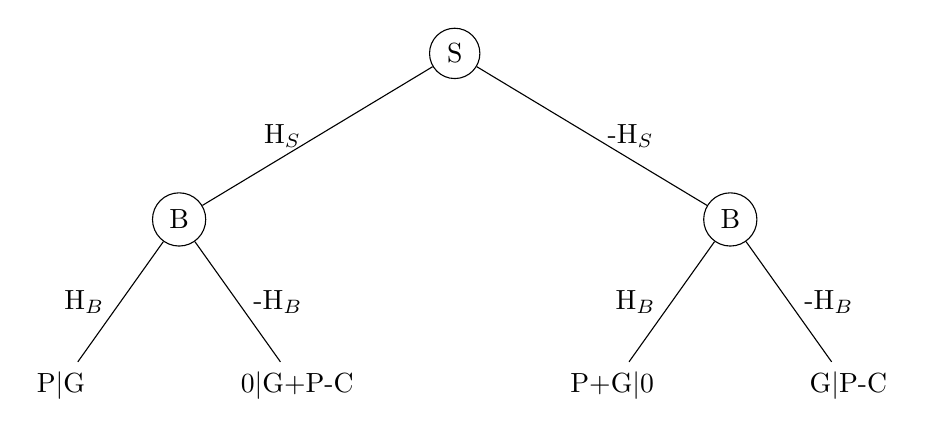
\begin{tikzpicture}[sibling distance=7cm,level distance=6em,every node/.style={shape=circle,align=center}]
      \node[draw]{S}
        child{node[draw]{B}
                child[sibling distance = 3cm]{node[shape = rectangle]{P$|$G} edge from parent node [left] {H$_B$}} 
                child[sibling distance = 3cm]{node[shape=rectangle]{0$|$G+P-C}edge from parent node [right] {-H$_B$}} edge from parent node [left] {H$_S$}} 
        child{node[draw]{B}
            child[sibling distance = 3cm]{node[shape=rectangle]{P+G$|$0}edge from parent node [left] {H$_B$}}
            child[sibling distance = 3cm]{node[shape = rectangle]{G$|$P-C}edge from parent node [right] {-H$_B$}}edge from parent node [right] {-H$_S$}};
\end{tikzpicture}

\begin{center}
\begin{tabular}{ c||c|c| }
& H$_B$ & -H$_B$   \\
\hline
\hline
H$_S$ & $P | G$ & $0 | G + P - C$  \\
\hline
-H$_S$ & $G + P | 0$ & $G | P - C$  \\ 
%\hline
%C$_S$ & $ G | P-C$ & $G + \frac{P}{2}  | \frac{P}{2}$  \\ 
\hline
\end{tabular}
\end{center}

The biggest possible payout for the Seller is if he can coerce the Buyer into sending him additional $\frac{P}{2}$ coins. This happens when the seller is choosing strategy C$_S$ and the buyer strategy -H$_B$.  It should be noted, that when the seller tries to coerce the buyer (C$_S$), it is actually his best option to comply (-H$_B$). This scenario is the Nash Equilibrium, because choosing a different strategy only results in a lower payoff for the player, if the other player is keeping his strategy.\newline
The Nash Equilibrium would result in a payoff of $G + \frac{P}{2}$ for the Buyer and a payoff of $\frac{P}{2}$ for the seller. The rational buyer would never initiate the trade, because this trade will always result in a loss, if the seller behaves rational.

\subsection{Seller Collateral}
Following protocol is proposed:
\begin{enumerate}
    \item Seller deposits collateral $C > P$ to the Smart Contract
    \item Buyer sends funds of amount $P$ to the seller 
    \item Seller sends the physical good to the Buyer
    \item Buyer receives the physical good and confirms it to the Smart Contract
    \item The Smart Contract releases the collateral of the Seller
\end{enumerate}
The collateral should incentivize the Seller to behave honestly and to ship the physical good to the buyer.
%Because of the collateral, behaving honestly should be the best strategy for the seller.
\minisec{Possible Strategies}
With this new protocol there are again new possible strategies. There is still the honest strategy for both players, where they behave according to the protocol description. With this strategy, the trade still unravels successfully.\newline
But there exist other strategies: The dishonest strategy is again not sending the resources. This strategy is still denoted as -H$_B$ (when the buyer does not send the coins) and -H$_S$ (when the seller does not send the physical good.\newline
The Buyer has also a unique opportunity: Since he decides what happens to the collateral, he can coerce the Seller into sending him extra resources. This strategy will be denoted C$_B$.  After receiving the physical good he can tell the Seller: "Either you send me back my payment $P$ or I will tell the Smart Contract that you did not send me the physical good." In this case it is best for S to comply, because $C > P$. \newline



\minisec{Payout}

\begin{tikzpicture}[sibling distance=7cm,level distance=6em,every node/.style={shape=circle,align=center}]
      \node[draw]{B}
        child{node[draw]{S}
                child[sibling distance = 7cm]{node[draw]{B}
                		child[sibling distance = 3cm]{node[shape = rectangle]{P$|$G} edge from parent node [left] {H$_B$}} 
                		child[sibling distance = 3cm]{node[shape=rectangle]{0$|$ G+P}edge from parent node [right] {C$_B$}} edge from parent node [left] {H$_S$}} 
                child[sibling distance = 7cm]{node[draw]{B}
                child[sibling distance = 3cm]{node[shape = rectangle]{G+P-C$|$0} edge from parent node [left] {H$_B$}} 
                child[sibling distance = 3cm]{node[shape=rectangle]{G$|$P}edge from parent node [right] {C$_B$}}edge from parent node [right] {-H$_S$}} edge from parent node [left] {H$_B$}} 
          child[sibling distance = 10cm]{node[shape = rectangle]{G$|$P}edge from parent node [right] {-H$_B$}};
\end{tikzpicture}

Normally there is another layer under C$_B$: Does S comply and send P or not? As already discussed, it is always better for the seller to send back the payment $P$ and recieve back his collateral $C$, because $C>P$. Should I put it in the tree? make it bigger and more difficult to read but completely correct.
\begin{center}
\begin{tabular}{ c||c|c|c| }
& H$_B$ & -H$_B$ & C$_B$  \\
\hline
\hline
H$_S$ & $P | G$ & $G | P$ & $0 | G + P$ \\
\hline
-H$_S$ & $P + G - C | 0$ & $G | P$ & $G | P$ \\ 
\hline
\end{tabular}
\end{center}
If B sends the coins (does not choose strategy -H$_B$), S has to make the following decision: Does he send the good (H$_S$) or not (-H$_S$)? We have to take into account, that B decides what happens with the collateral. \newline
%If S does not behave honestly (does not send the good), B can punish S by reporting 0 to the Smart contract. This means, that the collateral would not be given back to S.
What was designed to be an incentive for S to behave honestly, ended up as leverage for B over S. B can report 0 (and burn the collateral) even if S behaves honestly. 
%Therefore B can use this leverage to coerce S into giving him extra resources: “Give me C/2 coins or I will report 0 to the Smart Contract and burn your collateral.“
Since sending the good has no impact on the collateral (the rational buyer will always play strategy C$_B$ over H$_B$), it is best for S to not send the physical good (-H$_B$).
Because not Sending (-H$_S$) is the best strategy for the seller, it is best for B to not even send P and therefore not engage in the trade at all (-H$_B$).\newline
The Nash Equilibrium would be in nobody sending anything and the trade not happening.


\section{Two Side Collateral}
Following protocol is proposed:
\begin{enumerate}
    \item Seller  deposits collateral $C_1 > P$ to the Smart Contract
    \item Buyer  deposits collateral $C_2 > P$ to the Smart Contract
    \item Buyer sends Funds of amount $P$ to the Seller
    \item Seller sends physical good $G$ to the seller 
    \item Buyer receives the physical good and confirms it to the Smart Contract
    \item The Smart Contract releases the collateral of the Seller and the Buyer
\end{enumerate}

\minisec{Payout}

\begin{tikzpicture}[sibling distance=7cm,level distance=6em,every node/.style={shape=circle,align=center}]
      \node[draw]{B}
        child{node[draw]{S}
                child[sibling distance = 7cm]{node[draw]{B}
                		child[sibling distance = 3cm]{node[shape = rectangle]{P$|$G} edge from parent node [left] {1}} 
                		child[sibling distance = 3cm]{node[shape=rectangle]{P-C$_1|$G-C$_2$}edge from parent node [right] {0}} edge from parent node [left] {H$_S$}} 
                child[sibling distance = 7cm]{node[draw]{B}
                child[sibling distance = 3cm]{node[shape = rectangle]{G+P$|$0} edge from parent node [left] {1}} 
                child[sibling distance = 3cm]{node[shape=rectangle]{G+P-C$_1|$-C$_2$}edge from parent node [right] {0}}edge from parent node [right] {-H$_S$}} edge from parent node [left] {H$_B$}} 
          child[sibling distance = 10cm]{node[shape = rectangle]{G$|$P -C}edge from parent node [right] {-H$_B$}};
\end{tikzpicture}

\begin{equation}
    U_s(P) > U_s(nothing) 
\end{equation}
\newline
\chapter{Open Research/ Questions}

\chapter{Conclusion}
	
	
	%\bibliographystyle{}
	%\bibliography{}
	
	\appendix
\end{document}